\chapter{Set Theory}

    \minitoc

\section{Axiomatization}\label{section:axiomatization}
\subsection{ZFC}

    The following set of axioms and axiom schemata gives a foundation for axiomatic set theory whilst fixing a number of issues in naive set theory, where the notion of a set is taken for granted. This theory is called \textbf{Zermelo--Frenkel} set theory (ZF). When extended with the axiom of choice (see further on), it is called ZFC, where the C stand for `choice'.

    \begin{axiom}[Power set]\index{power!set}\label{set:power_set_axiom}
        \begin{gather}
            \forall x:\exists y:\forall z\bigl(z\in y\iff\forall w(w\in z\implies w\in x)\bigr)
        \end{gather}
        The set $y$ is called the power set $P(x)$ or $2^x$ of $x$.
    \end{axiom}

    \begin{axiom}[Extensionality]\index{extensionality}
        \begin{gather}
            \forall x,y:\forall z\bigl(z\in x\iff z\in y\bigr)\implies x=y
        \end{gather}
        This axiom allows to compare two sets based on their elements, i.e.~two sets are (strictly) equal if and only if they have the same elements.
    \end{axiom}
    \begin{remark}
        As will be made clear throughout this document, strict equality as in the extensionality axiom is often not what one cares about in practice. \textit{Equivalence} and \textit{isomorphism} will be the practically relevant notions.
    \end{remark}

    \begin{axiom}[Regularity\footnotemark]\index{regularity}
        \footnotetext{Also called the \textbf{axiom of foundation}.}
        \begin{gather}
            \forall x:(\exists z\in x)\implies(\exists a\in x)\land\neg(\exists b\in a:b\in x)
        \end{gather}
        This axiom says that for every nonempty set $x$, one can find an element $a\in x$ such that $x$ and $a$ are disjoint. Among other things, this axiom implies that no set can contain itself.
    \end{axiom}

    The following axiom is technically not an axiom but an axiom schema, i.e.~for every predicate $\varphi$, one obtains an axiom.
    \begin{axiom}[Specification]\index{specification}
        \begin{gather}
            \forall w_1,\ldots,w_n,A:\exists B:\forall x\bigl[x\in B\iff\bigl(x\in A\land\varphi(x,w_1,\ldots,w_n,A)\bigr)\bigr]
        \end{gather}
        This axiom (schema) says that, for every set $x$, one can build another set of elements in $x$ that satisfy a given predicate. By the axiom of extensionality, this subset $B\subseteq A$ is unique.
    \end{axiom}
    \begin{notation}[Set builder notation]\index{set!builder notation}
        The sets constructed through the axiom of specification are often denoted as follows:
        \begin{gather}
            B=\{x\in A\mid\phi(x)\}\,,
        \end{gather}
        where the parameters $w_1,\ldots,w_n$ were suppressed for conciseness.
    \end{notation}

\subsection{Material set theory}\index{set theory!material}

    ZF(C) is an instance of \textit{material set theory}. Every element of a set is itself a set and, hence, possesses some kind of internal structure.

    \newdef{Pure set}{\index{pure!set}
        A set $U$ such that, for every sequence
        \begin{gather}
            x_n\in x_{n-1}\in\cdots\in x_1\in U\,,
        \end{gather}
        all elements $x_i$ are also sets.
    }
    \newdef{Urelement\footnotemark}{\index{urelement}\index{atom}
        \footnotetext{Sometimes called an \textbf{atom}.}
        An object that is not a set.
    }

    \todo{COMPLETE}

\subsection{Structural set theory}\index{set theory!structural}

    In contrast to material set theory, the fundamental notions in this theory are the relations between sets. An element of a set does not have any internal structure and only becomes relevant if one specifies extra structure (given by relations) on the sets. This implies that elements of sets are not sets themselves. In fact, this would be a meaningless statement since, by default, they lack any internal structure. Even stronger, it is meaningless to compare two elements if one does not provide relations or extra structure on the sets.

    \todo{COMPLETE}

\subsection{\texorpdfstring{ETCS $\clubsuit$}{ETCS}}

    \sremark{ETCS is the abbreviation of `Elementary Theory of the Category of Sets'.}

    \begin{axiom}
        The category of sets is a \textit{well-pointed (elementary) topos} (see \cref{chapter:topos}).
    \end{axiom}

    \todo{COMPLETE}

\subsection{Universes}\label{section:universes}

    To be able to talk about sets without running into problems such as \textit{Russel's paradox}, where one needs (or wants) to talk about the collection of all things satisfying a certain condition, one can introduce the concept of a `universal set' or `universe (of discourse)'. This set takes the place of the `collection of things' and all operations act within this universe.

    \newdef{Grothendieck universe}{\index{Grothendieck!universe}
        A pure set $U$ satisfying the following conditions:
        \begin{enumerate}
            \item\textbf{Transitivity}: If $x\in U$ and $y\in x$, then $y\in U$.
            \item\textbf{Power set}: If $x\in U$, then $P(x)\in U$.
            \item\textbf{Pairing}: If $x,y\in U$, then $\{x,y\}\in U$.
            \item\textbf{Unions}: If $I\in U$ and $\{x_i\}_{i\in I}\subset U$, then $\bigcup_{i\in I}x_i\in U$.
        \end{enumerate}
    }

\section{Finite sets}

    \newdef{Bishop finiteness}{\index{finite!set}\index{Bishop|see{finite set}}
        A set $S$ is said to be (Bishop) finite if there exists a bijection $S\cong[n]$ for some $n\in\mathbb{N}$.
    }

    In ZFC, any other reasonable definition of finite sets will be equivalent to the one above. However, in constructive mathematics, this is not true anymore. Because the \textit{internal logic} of \textit{elementary topoi} (see \cref{chapter:topos}) is constructive, some more information is given here.

    \newdef{Kuratowski finiteness}{\index{Kuratowski|see{finite set}}
        A set $S$ is said to be Kuratowski finite or \textbf{finitely indexed set} if there exists a surjection $[n]\twoheadrightarrow S$ for some $n\in\mathbb{N}$.
    }

    \newdef{Dedekind finiteness}{\index{Dedekind|see{finite set}}
        A set $S$ is said to be Dedekind finite if any injection $S\hookrightarrow S$ is a bijection.
    }

    \todo{COMPLETE}

\section{Real numbers}\index{real numbers}

    \begin{axiom}[Ordering]
        The set of real numbers is an \textit{ordered field} (see \cref{algebra:field}).
    \end{axiom}
    \begin{axiom}[Dedekind completeness]\index{Dedekind!completeness}\label{set:dedekind_completeness}
        Every nonempty subset of $\mathbb{R}$ that is bounded from above has a \textit{supremum} (see \cref{set:supremum} and \cref{set:complete_lattice}).
    \end{axiom}

    \begin{axiom}
        The rational numbers form a subset of the real numbers: $\mathbb{Q}\subset\mathbb{R}$.
    \end{axiom}

    \begin{remark}
        There is only one way (up to isomorphisms) to extend the field of rational numbers to the field of reals such that it satisfies the previous axioms.
    \end{remark}

    \newdef{Extended real line}{\label{calculus:extended_real_line}
        \begin{gather}
            \overline{\mathbb{R}} := \mathbb{R}\cup\{-\infty,\infty\} \equiv [-\infty,\infty]
        \end{gather}
    }

\section{Set operations}

    \newdef{Cartesian product}{\index{product}
        Let $X,Y$ be two sets. Their (Cartesian) product is defined as follows:
        \begin{gather}
            X\times Y := \{(x,y)\mid x\in X\land y\in Y\}\,.
        \end{gather}
    }

    \newdef{Symmetric difference}{\index{symmetric!difference}\label{set:symmetric_difference}
        \begin{gather}
            A\Delta B := (A\backslash B)\cup(B\backslash A)
        \end{gather}
    }

    \newdef{Diagonal}{\index{diagonal}
        The diagonal of a set $X$ is defined as follows:
        \begin{gather}
            \Delta_X := \bigl\{(x,x)\in X\times X\bigm\vert x\in X\bigr\}\,.
        \end{gather}
    }

    \newdef{Complement}{\index{complement}\label{set:complement}
        Let $\Omega$ be the universe of discours (\cref{section:universes}) and consider $X\subseteq\Omega$. The complement of $X$ is defined as follows:
        \begin{gather}
            X^c := \Omega\backslash X\,.
        \end{gather}
    }

    \newformula{de Morgan's laws}{\index{de Morgan!law}
        \begin{gather}
            \label{set:de_morgan_union}
            \left(\bigcup_iX_i\right)^c = \bigcap_iX_i^c
        \end{gather}
        \begin{gather}
            \label{set:de_morgan_intersection}
            \left(\bigcap_iX_i\right)^c = \bigcup_iX_i^c
        \end{gather}
    }

    \newdef{Relation}{\index{relation}\label{set:relation}
        A relation between two sets $X$ and $Y$ is a subset of the Cartesian product $X\times Y$. A relation on $X$ is then simply a subset of $X\times X$. This definition can easily be extended to $n$-ary relations by working with subsets of $n$-fold products.
    }

    \newdef{Converse relation}{\index{converse}\label{set:converse}
        Consider a relation $R\subseteq X\times Y$. The converse relation $R^t$ is defined as follows:
        \begin{gather}
            R^t := \bigl\{(y,x)\in Y\times X\bigm\vert(x,y)\in R\bigr\}\,.
        \end{gather}
    }
    \newdef{Composition of relations}{\index{composition!of relations}\label{set:relational_composition}
        Consider two relations $R\subseteq X\times Y$ and $S\subseteq Y\times Z$ between three sets $X,Y$ and $Z$. The composition $S\circ R$ is defined as follows:
        \begin{gather}
            S\circ R := \bigl\{(x,z)\in X\times Z\bigm\vert\exists y\in Y:(x,y)\in R\land(y,z)\in S\bigr\}.
        \end{gather}
    }

\section{Functions}
\subsection{(Co)domain}

    \newdef{Domain}{\index{domain}\label{set:domain}
        Let $f:X\rightarrow Y$ be a function. The set $X$ is called the domain of $f$.
    }
    \begin{notation}
        The domain of $f$ is denoted by $\mathrm{dom}(f)$.
    \end{notation}

    \newdef{Support}{\index{support}
        Let $f:X\rightarrow\mathbb{R}$ be a function. The support of $f$ is defined as the set of points where $f$ is nonzero.
    }
    \begin{notation}
        The support of $f$ is denoted by $\supp(f)$.
    \end{notation}

    \begin{notation}\label{set:function_set}
        Let $X,Y$ be two sets. The set of functions $f:X\rightarrow Y$ is denoted by $Y^X$ or $\mathrm{Map}(X,Y)$. (See also \cref{cat:exponential_object} for a generalization.)
    \end{notation}

    \newdef{Codomain}{\index{co-!domain}
        Let $f:X\rightarrow Y$ be a function. The set $Y$ is called the codomain of $f$.
    }
    \newdef{Image}{\index{image}
        Let $f:X\rightarrow Y$ be a function. The following subset of $Y$ is called the image of $f$:
        \begin{gather}
            \im(f):=\{y\in Y\mid\exists x\in X:f(x) = y\}\,.
        \end{gather}
    }
    \sremark{Some authors use the notions of codomain and image interchangeably.}

    \newdef{Level set}{\index{level!set}\index{fibre}\index{pre-!image}\label{set:level_set}
        Consider a function $f:X\rightarrow\mathbb{R}$. The following set is called the level set of $f$ at $c\in\mathbb{R}$:
        \begin{gather}
            f^{-1}(c) := \{x\in X\mid f(x) = c\}\,.
        \end{gather}
        For $X=\mathbb{R}^2$ the level sets are called \textbf{level curves} and for $X=\mathbb{R}^3$ they are called \textbf{level surfaces}. More generally, for functions $f:X\rightarrow Y$, one calls $f^{-1}(y)$ the \textbf{preimage} or \textbf{fibre} of $f$ over $y$.
    }

\subsection{Functions}

    \newdef{Injective}{\index{injective}\index{one-to-one|see{injective}}\label{set:injective}
        A function $f:A\rightarrow B$ is said to be injective or \textbf{one-to-one} if the following condition is satisfied:
        \begin{gather}
            \forall a,a'\in A:f(a)=f(a')\implies a=a'\,.
        \end{gather}
    }
    \newnot{Injective function}{\[f:A\hookrightarrow B\]}

    \newdef{Surjective}{\index{surjective}\index{onto|see{surjective}}\label{set:surjective}
        A function $f:A\rightarrow B$ is said to be surjective or \textbf{onto} if the following condition is satisfied:
        \begin{gather}
            \forall b\in B:\exists a\in A:f(a) = b\,.
        \end{gather}
    }
    \newnot{Surjective function}{\[f:A\twoheadrightarrow B\]}

    \newdef{Bijection}{\index{bijection}
        A function that has an inverse. Equivalently, a function that gives a one-to-one correspondence between the elements of the domain and those of the codomain.
    }
    \newnot{Isomorphic sets}{
        \[X\cong Y\]
    }

    \begin{theorem}[Cantor--Bernstein--Schr\"oder]\index{Cantor--Bernstein--Schr\"oder}\label{set:CBS_theorem}
        Consider two sets $A,B$. If there exist injections $A\hookrightarrow B$ and $B\hookrightarrow A$, there exists a bijection $A\cong B$.
    \end{theorem}

    \newdef{Involution}{\index{involution}\label{set:involution}
        A function $f:A\rightarrow A$ such that $f^2=\mathbbm{1}_A$, i.e.~$f$ is its own inverse. Every involution is, in particular, a bijection.
    }

\section{Collections}
\subsection{Families and filters}\label{section:collections}

    \newdef{Power set}{\index{power!set}\label{set:power_set}
        Let $X$ be a set. The power set is defined as the set of all subsets of $X$ and is (often) denoted by $P(X)$ or $2^X$. The existence of this set is enforced by the power set axiom (\cref{set:power_set_axiom}).
    }
    \result{All sets are elements of their power set: $X\in P(X)$.}

    \newdef{Collection}{\index{collection}\index{index!set}
        A collection of elements of a set $X$ is a subset of $X$. Often, this collection is indexed by some \textbf{index set} $I$, in which case it is often denoted as $\{x_i\}_{i\in I}\subseteq X$.
    }
    \newdef{Family}{\index{family}\index{index!set}
        Let $X,I$ be two sets. A family of elements of $X$ with \textbf{index set} $I$ is a function $f:I\rightarrow X$. A family with index set $I$ is often denoted by $(x_i)_{i\in I}$. In contrast to collections, a family can contain multiple copies of the same element.
    }

    \todo{CHECK COMPENDIUM TO GET NOTATIONS STRAIGHT}

    \newdef{Helly family}{\index{Helly!family}\label{set:helly_family}
        A Helly family of order $k\in\mathbb{N}$ is a pair $(X,F)$ with $F\subset P(X)$ such that for every finite $G\subset F$:
        \begin{gather}
            \bigcap_{V\in G}V = \emptyset\implies\exists H\subseteq G: \left(\bigcap_{V\in H}V = \emptyset\right)\land\Bigl(|H|\leq k\Bigr)\,.
        \end{gather}
        A Helly family of order 2 is sometimes said to have the \textbf{Helly property}.

        \todo{WHERE IS THIS NEEDED?}
    }

    \newdef{Cover}{\index{cover}\label{set:cover}
        A cover of a set $X$ is a collection of sets $\{V_i\}_{i\in I}\subseteq P(X)$ such that:
        \begin{gather}
            \bigcup_{i\in I}V_i=X\,.
        \end{gather}
    }

    \newdef{Partition}{\index{partition}
        A  partition of $X$ is a collection of disjoint subsets $\{A_i\}_{i\in I}\subset P(X)$ such that $\bigcup_{i\in I}A_i=X$, i.e.~it is a disjoint cover.
    }
    \newdef{Refinement}{\index{refinement}
        Let $P$ be a partition of $X$. A refinement $P'$ of $P$ is a collection of subsets such that every $A\in P$ can be written as a disjoint union of elements in $P'$. It follows that every refinement is also a partition.
    }

    \newdef{Filter}{\index{filter}\label{set:filter}
        Let $X$ be a set. A family $\mathcal{F}\subseteq P(X)$ is a filter on $X$ if it satisfies the following conditions:
        \begin{enumerate}
            \item\textbf{Nonemptiness}: $\emptyset\not\in\mathcal{F}$.
            \item\textbf{Downward closure}: $\forall A,B \in\mathcal{F}:A\cap B\in\mathcal{F}$.
            \item\textbf{Isotony}: if $A\in\mathcal{F}$ and $A\subseteq B$, then $B\in\mathcal{F}$.
        \end{enumerate}
    }

    \newdef{Filtration}{\index{filtration}\label{set:filtration}
        Consider a set $X$ together with a collection of subsets $\{F_i\}_{i\in I}$ indexed by a \textit{totally ordered set} $I$ (see \cref{set:total_order}). The collection is said to be a filtration of $X$ if
        \begin{gather}
            i\leq j\implies F_i\subseteq F_j\,.
        \end{gather}
        A filtration is said to be \textbf{exhaustive} if $\bigcup_{i\in I}F_i=X$ and \textbf{separated} if $\bigcap_{i\in I}F_i=\emptyset$.
    }
    \newdef{Associated grading}{\index{graded!object}
        When one can define \textit{quotient objects}, every filtration $\{F_i\}_{i\in I}$ of $X$ defines an associated graded object $\{G_i := F_i/F_{i-1}\}_{i\in I}$.
    }

\subsection{Algebra of sets}

    \newdef{Algebra of sets}{\index{algebra!of sets}\index{field!of sets|see{algebra}}\index{Boolean!algebra}\label{set:algebra_of_sets}
        A collection $\mathcal{F}\subset P(X)$ is a called an algebra over $X$ if it satisfies the following conditions:
        \begin{enumerate}
            \item\textbf{Totality}: $X\in\mathcal{F}$,
            \item\textbf{Closed under complements}: $\forall E\in\mathcal{F}:E^c\in\mathcal{F}$, and
            \item\textbf{Closed under finite unions}: $\forall E,E'\in\mathcal{F}:E\cup E'\in\mathcal{F}$.
        \end{enumerate}
        The pair $(X,\mathcal{F})$ is also called a \textbf{field of sets} or \textbf{concrete Boolean algebra}.
    }

    Extending this definition to closure under countable unions gives another common notion.
    \newdef{$\sigma$-algebra}{\index{$\sigma$!algebra}\index{measurable}\label{set:sigma_algebra}
        A collection $\Sigma\subset P(X)$ is called a $\sigma$-algebra over a set $X$ if it satisfies the following conditions:
        \begin{enumerate}
            \item\textbf{Totality}: $X\in\Sigma$,
            \item\textbf{Closed under complements}: $\forall E\in\Sigma: E^c\in\Sigma$, and
            \item\textbf{Closed under countable unions}: $\forall\{E_n\}_{n\in\mathbb{N}}\subset\Sigma:\bigcup_{n=1}^{+\infty}E_n\in\Sigma$.
        \end{enumerate}
        The pair $(X,\Sigma)$ is called a \textbf{measurable space}. The elements $E\in\Sigma$ are called \textbf{measurable sets}.
    }
    \begin{remark}
        Conditions 1 and 2 imply that both $\sigma$-algebra and fields of sets always contain the empty set. Conditions 2 and 3, together with de Morgan's laws~\eqref{set:de_morgan_union} and~\eqref{set:de_morgan_intersection}, imply that a $\sigma$-algebra is also closed under countable intersections and, analogously, that a field of sets is closed under finite intersections.
    \end{remark}

    \begin{property}[Intersections]
        The intersection of a collection of $\sigma$-algebras is again a $\sigma$-algebra.
    \end{property}

    \newdef{Generated $\sigma$-algebras}{\label{set:generated_sigma_algebra}
        A $\sigma$-algebra $\mathcal{G}$ is said to be generated by a collection of sets $\mathcal{A}$ if
        \begin{gather}
            \mathcal{G} = \bigcap\{\mathcal{F}\mid\mathcal{F}\text{ is a } \sigma\text{-algebra that contains }\mathcal{A}\}\,.
        \end{gather}
        Equivalently, it is the smallest $\sigma$-algebra containing $\mathcal{A}$.
    }
    \begin{notation}\label{set:notation:generated_sigma_algebra}
        The $\sigma$-algebra generated by a collection of sets $\mathcal{A}$ is often denoted by $\sigma(\mathcal{A})$.
    \end{notation}

    \newdef{Product $\sigma$-algebras}{\label{set:product_of_sigma_algebras}
        The product $\sigma$-algebra $\mathcal{F}_1\otimes\mathcal{F}_2$ on $X_1\times X_2$ can be defined in the following equivalent ways:
        \begin{itemize}
            \item $\mathcal{F}$ is generated by $\{A_1\times\Omega_2\mid A_1\in\mathcal{F}_1\}\cup\{\Omega_1\times A_2\mid A_2\in\mathcal{F}_2\}$.
            \item $\mathcal{F}$ is generated by $\{A_1\times A_2\mid A_1\in\mathcal{F}_1\land A_2\in\mathcal{F}_2\}$.
        \end{itemize}
    }

    \newdef{Monotone class}{\index{monotone!class}
        A collection of sets $\mathcal{A}$ that has the following two properties:
        \begin{enumerate}
            \item For every increasing sequence $A_1\subset A_2\subset\cdots$ : $\bigcup_{n=1}^{+\infty}A_n\in\mathcal{A}$.
            \item For every decreasing sequence $A_1\supset A_2\supset\cdots$ : $\bigcap_{n=1}^{+\infty}A_n\in\mathcal{A}$.
        \end{enumerate}
    }

    \begin{theorem}[Monotone class theorem]\label{set:monotone_class}
        Let $\mathcal{A}$ be an algebra of sets. If $\mathcal{G}_{\mathcal{A}}$ is the smallest monotone class containing $\mathcal{A}$, it coincides with the $\sigma$-algebra generated by $\mathcal{A}$.
    \end{theorem}

\section{Ordered sets}\index{order}\label{section:ordered_sets}
\subsection{Posets}

    \newdef{Partially ordered set}{\index{poset}\index{pre-!order|see{order}}\label{set:poset}
        A set $P$ equipped with a binary relation $\leq$ is called a partially ordered set (or \textbf{poset}) if the following 3 conditions are satisfied for all elements $x,y,z\in P$:
        \begin{enumerate}
            \item\textbf{Reflexivity}: $x\leq x$,
            \item\textbf{Antisymmetry}: $x\leq y\land y\leq x\implies x=y$, and
            \item\textbf{Transitivity}: $x\leq y\land y\leq z\implies x\leq z$.
        \end{enumerate}
        If the antisymmetry condition is dropped, a \textbf{preorder} is obtained.
    }

    \newdef{Order-preserving map}{\index{monotone!function}\index{order!-preserving}
        A function $f:(P,\leq)\rightarrow(P',\preceq)$ of posets such that $x\leq y\implies f(x)\preceq f(y)$ for all $x,y\in P$. These functions are also said to be \textbf{monotone}.
    }

    \newdef{Hasse diagram}{\index{Hasse diagram}
        Consider a finite poset $(P,\leq)$. A Hasse diagram for $P$ is a \textit{graph} where the vertices are given by the elements of $P$ and two vertices $x,y$ are connected upwardly if and only if $x\leq y$ in $P$.
    }
    \begin{example}
        Consider the power set of $\{0,1\}$ with its canonical poset structure. A Hasse diagram of this poset is
        \begin{gather*}
            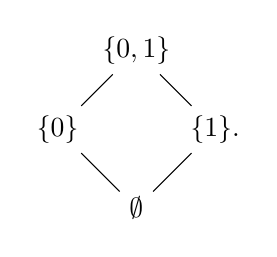
\begin{tikzpicture}
                \node (01) at (0, 0) {$\{0,1\}$};
                \node (0) at (-1, -1) {$\{0\}$};
                \node (1) at (1, -1) {$\{1\}.$};
                \node (empty) at (0, -2) {$\emptyset$};
                \draw (empty) -- (0) -- (01);
                \draw (empty) -- (1) -- (01);
            \end{tikzpicture}
        \end{gather*}
    \end{example}

    \newdef{Totally ordered set}{\index{totality}\label{set:total_order}
        A poset $P$ with the property that for all $x,y\in P$, either $x\leq y$ or $y\leq x$. This property is called \textbf{totality}.
    }
    \newdef{Strict total order}{
        A nonstrict order $\leq$ has an associated strict order $<$ that satisfies $x<y\iff x\leq y\land x\neq y$.
    }

    \newdef{Linear order}{
        A binary relation $<$ on a set $P$ satisfying the following conditions for all $x,y,z\in P$:
        \begin{enumerate}
            \item\textbf{Irreflexivity}: $x\not<x$,
            \item\textbf{Asymmetry}: $x<y\implies y\not<x$,
            \item\textbf{Transitivity}: $x<y\land y<z\implies x<z$,
            \item\textbf{Comparison}: $x<z\implies x<y\lor y<z$, and
            \item\textbf{Connectedness}: $x\not<y\land y\not<x\implies x=y$.
        \end{enumerate}
    }
    \remark{By negation, one can freely pass between linear orders and total orders. However, without the law of the excluded middle, there exists no bijection between them.}

    \newdef{Supremum}{\index{supremum}\label{set:supremum}
        The supremum $\sup(P)$ of a poset $P$ is the least upper bound of $P$.
    }
    \newdef{Infimum}{\index{infimum}\label{set:infimum}
        The infimum $\inf(P)$ of a poset $P$ is the greatest lower bound of $P$.
    }

    \newdef{Maximum}{\index{maximum}\label{set:maximum}
        If $\sup(P)\in P$, the supremum is called the maximum of $P$. This is denoted by $\max(P)$.
    }
    \newdef{Minimum}{\index{minimum}\label{set:minimum}
        If $\inf(P)\in P$, the supremum is called the minimum of $P$. This is denoted by $\min(P)$.
    }

    \newdef{Chain}{\index{chain}\label{set:chain}
        A totally ordered subset of a poset.
    }
    \begin{theorem}[Zorn's lemma\footnotemark]\index{Zorn's lemma}\label{set:zorns_lemma}
        \footnotetext{This theorem is equivalent to the \textit{axiom of choice}.}
        Let $(P,\leq)$ be a poset. If every chain in $P$ has an upper bound in $P$, then $P$ has a maximal element.
    \end{theorem}

    \newdef{Directed\footnotemark\ set}{\index{directed set}\index{filtered set|see{directed set}}\label{set:directed_set}
        \footnotetext{Sometimes called a \textbf{filtered} set or \textbf{upward} directed set. \textbf{Downward} directed sets are analogously defined with a lower bound for every two elements.}
        A set $P$ equipped with a preorder $\leq$ with the additional property that every 2-element subset has an upper bound, i.e.~for every two elements $x,y\in P$, there exists an element $z\in P$ such that $x\leq z\land y\leq z$.
    }
    \newdef{Net}{\index{net}\label{set:net}
        A net on a set $X$ is a subset of $X$ indexed by a directed set $I$.
    }

    \newdef{Cut}{\index{cut}\index{Dedekind!cut}\index{union!ordered}
        Let $(P,\leq)$ be a totally ordered set. A cut or \textbf{decomposition} of $P$ is a pair $(A,B)$ of disjoint subsets such that $P=A\cup B$ in the ordered sense, i.e.~every element of $A$ is smaller than every element of $B$. Cuts can be classified as follows:
        \begin{itemize}
            \item\textbf{Jumps}: $A$ has a greatest element and $B$ has a least element.
            \item\textbf{Dedekind cut}: Either $A$ has a greatest element and $B$ has no least element or $A$ has no greatest element, but $B$ has a least element.
            \item\textbf{Gap}: $A$ has no greatest element and $B$ has no least element.
        \end{itemize}
    }

    The notion of a filter on a set $X$ (\cref{set:filter}) is a specific example of a more general notion, where the underlying poset is the power set of $X$.
    \newdef{Filter}{\index{filter}\index{ultrafilter}\label{set:ultrafilter}
        Let $X$ be a poset. A filter on $X$ is a subset $\mathcal{F}\subseteq X$ such that:
        \begin{enumerate}
            \item\textbf{Nonemptiness}: $\mathcal{F}\neq\emptyset$,
            \item\textbf{Downward closure}: $\forall x,y\in\mathcal{F}:\exists z\in\mathcal{F}:z\leq x\land z\leq y$, and
            \item\textbf{Isotony}: If $x\in\mathcal{F}$ and $x\leq y$, then $y\in\mathcal{F}$.
        \end{enumerate}
        If there exists no strictly greater filter $\mathcal{F}\subset\mathcal{F}'$, then $\mathcal{F}$ is called an \textbf{ultrafilter}.
    }

    The following theorem is independent of the ZF axioms, but strictly weaker than the \textit{axiom of choice}.
    \begin{theorem}[Ultrafilter lemma]
        Every proper filter on a set is contained in an ultrafilter.
    \end{theorem}

\subsection{\difficult{Ordinals}}

    \newdef{Well-ordering}{\index{well-!order}\index{well-!founded}
        A \textbf{well-founded} linear order, i.e.~a linear order such that every nonempty subset has a minimal element.
    }

    \newdef{Ordinal number}{\index{number!ordinal}\label{set:ordinal}
        Consider the class of all well-ordered sets. An ordinal (type or rank) is an isomorphism class of well-ordered sets. The class of ordinals is itself well ordered by inclusion of `initial segments'.

        However, this definition gives problems within the ZF(C) framework of set theory, since these equivalence classes are proper classes and not sets. To overcome this problem, one can use a different approach. By using a well-defined construction, one can, for every class, select a particular representative and call this representative the \textbf{ordinal number} of all well-ordered sets isomorphic to it.
    }

    The most common construction is the one by \indexauthor{von Neumann}. For every well-ordered set $W$, there exists a function
    \begin{gather}
        W\rightarrow P(W):w\mapsto W_{\leq w}:=\{w'\in W\mid w'\leq w\}
    \end{gather}
    that restricts to an order isomorphism on its image. This leads to the following definition.
    \newdef{von Neumann ordinal}{\index{von Neumann!ordinal}
        A set that is strictly well ordered by membership and such that every element is also a subset.

        The first finite von Neumann ordinals are given as an example:
        \begin{itemize}
            \item $0 := \emptyset$,
            \item $1 := \{0\} = \{\emptyset\}$,
            \item $2 := \{0, 1\} = \{\emptyset,\{\emptyset\}\}$, and so on.
        \end{itemize}
    }

    \begin{property}
        Every ordinal type is uniquely order-isomorphic to an ordinal number. Consequently, every order-preserving isomorphism between an order type and itself is the identity.
    \end{property}

    \newdef{Successor}{\index{successor}\index{limit!ordinal|see{ordinal}}
        Every ordinal number $\alpha$ has a \textbf{successor} $\alpha^+$. Using the von Neumann definition, this is simply $\alpha^+ := \alpha\cup\{\alpha\}$. An ordinal that is not the successor of another ordinal number is called a \textbf{limit ordinal}.
    }
    \newdef{Regular ordinal}{\index{regular!ordinal}
        A limit ordinal $\alpha$ that is not the limit of a set of smaller ordinals with order type less than $\alpha$.
    }

    \begin{property}[Burali--Forti paradox]\index{Burali--Forti paradox}
        The class of all ordinals (and, by extension, the class of all well-ordered sets) is not a set.
    \end{property}

\subsection{\difficult{Cardinals}}

    There also exist numbers representing the sizes of sets, the \textbf{cardinal numbers}. These `numbers' should satisfy the following conditions:
    \begin{enumerate}
        \item Every set has a well-defined cardinality.
        \item Every cardinal number is the cardinality of some set.
        \item Bijective sets have the same cardinality.
    \end{enumerate}
    Guided by these conditions, one could naively use the following definition.
    \newdef{Cardinal number\footnotemark}{\index{number!cardinal}
        \footnotetext{Also called the \textbf{cardinality} of a set.}
        An isomorphism class of sets (under bijections).
    }

    However, similar to the problem encountered for ordinals above, these classes are not sets. To solve this, one can also use a similar trick and select a specific representative. For cardinals, the following choice is common.
    \newadef{Cardinal number}{
        The cardinal number of a set is the smallest ordinal rank of any well-order on it, i.e.~any ordinal number bijective to it.\footnote{The \textit{well-ordering theorem} (if assumed) assures that this definition coincides with the naive one above.} The cardinal numbers inherit a well-ordering from the ordinal numbers.
    }

    \begin{remark}[Ordering]
        The Cantor--Bernstein--Schr\"oder theorem~\ref{set:CBS_theorem} induces a partial ordering on cardinal numbers. However, without the axiom of choice this can never be a total ordering. This problem is also apparent in the above definition since the ordinal rank of sets is used together with the \textit{well-ordering theorem}, which is equivalent to the axiom of choice.
    \end{remark}

    Similar to ordinal numbers, one can also define successors of cardinal numbers.
    \newdef{Successor}{\index{successor}
        Given a cardinal $\kappa$, its successor $\kappa^+$ is defined as the smallest cardinal greater than $\kappa$.
    }
    \begin{remark}
        It should be noted that the successor of a cardinal number is not necessarily the same as its successor as an ordinal number (in fact, this is only the case for finite cardinals).
    \end{remark}

    \newdef{Regular cardinal}{\index{regular!cardinal}\label{set:regular_cardinal}
        An infinite cardinal $\kappa$ such that there exists no set of cardinality $\kappa$ that is the union of less than $\kappa$ subsets of cardinality less than $\kappa$:
        \begin{gather}
            \left(\kappa=\sum_{i\in I}\lambda_i\right)\land\bigl(\forall i\in I:\lambda_i<\kappa\bigr)\implies|I|\geq\kappa.
        \end{gather}
    }

    The following theorem can easily be proven by a diagonal argument.
    \begin{theorem}[Cantor]\index{Cantor}
        Let $S$ be a set of cardinality $\kappa$. The power set $P(S)$ has cardinality strictly greater than $\kappa$.
    \end{theorem}

\subsection{Lattices}

    \newdef{Semilattice}{\index{join}\index{meet}
        A poset $(P,\leq)$ for which every 2-element subset has a supremum, called the \textbf{join}, is called a \textbf{join-semilattice}. Similarly, a poset $(P,\leq)$ for which every 2-element subset has an infimum, called the \textbf{meet}, is called a \textbf{meet-semilattice}.
    }
    \begin{notation}
        The join of $\{x,y\}$ is denoted by $x\land y$. The meet of $\{x,y\}$ is denoted by $x\lor y$.
    \end{notation}
    \newdef{Lattice}{\index{lattice}
        A poset that is both a join- and a meet-semilattice.
    }

    The above definition also allows for a purely algebraic formulation (in this case, some authors might speak about \textbf{lattice-ordered sets}).
    \newadef{Lattice}{\index{absorption!law}\index{lattice}
        A lattice is an algebraic structure that admits operations $\land,\lor$ that satisfy the following conditions:
        \begin{enumerate}
            \item Both $\land$ and $\lor$ are idempotent, commutative and associative.
            \item The operations satisfy the \textbf{absorption laws}:
            \begin{gather}
                x\lor(x\land y)=x \qquad\qquad\qquad x\land(x\lor y)=x.
            \end{gather}
        \end{enumerate}
        To go from this definition to the order-theoretic one, define the partial order
        \begin{gather}
            x\leq y\iff x\land y=x\,.
        \end{gather}
        There exists an equivalent relation for the join.
    }

    \newdef{Complete lattice}{\index{complete!lattice}\index{adjoint functor theorem}\index{Dedekind!completeness}\label{set:complete_lattice}
        A lattice is said to be $\sigma$-complete (resp.~complete) if it admits all\footnote{When working with \textit{categories} (see \cref{chapter:cat}), this has to be restricted to `all small joins/meets' or, equivalently, the index category should be a set.} countable (resp.~all) joins. It can be proven that complete lattices also admit all meets (as a special case of the \textit{Adjoint Functor Theorem}~\ref{cat:adjoint_functor_theorem}). If only bounded (from above) subsets admit a join, the lattice is said to be \textbf{Dedekind-complete}. 
    }

    \newdef{Bounded lattice}{\index{lattice!bounded}
        A lattice $(L,\leq,\land,\lor)$ that contains a greatest element (denoted by $\top$ or 1) and a smallest element (denoted by $\bot$ or 0) such that
        \begin{gather}
            \bot\leq x\leq\top
        \end{gather}
        for all $x\in P$. These elements are the identities for the join and meet operations:
        \begin{gather}
            x\land\top=x\qquad\qquad\qquad x\lor\bot=x\,.
        \end{gather}
    }

    \newdef{Frame}{\index{frame!set theory}\index{distributivity}\label{set:frame}
        A complete lattice $(L,\leq,\land,\lor)$ for which the \textbf{infinite distributivity law} is satisfied:
        \begin{gather}
            y\land\left(\bigvee_{i\in I}x_i\right) = \bigvee_{i\in I}\left(y\land x_i\right)\,.
        \end{gather}
    }

    \newdef{Distributive lattice}{\index{lattice!distributive}\index{modular|seealso{lattice}}\index{lattice!modular}
        A lattice $(L,\leq,\land,\lor)$ such that
        \begin{gather}
            a\land(b\lor c) = (a\land b)\lor(a\land c)
        \end{gather}
        and\footnote{This second condition is actually a consequence of the first.}
        \begin{gather}
            a\lor(b\land c) = (a\lor b)\land(a\lor c)
        \end{gather}
        for all $a,b,c\in L$. If only
        \begin{gather}
            a\leq c\implies a\lor(b\land c)=(a\lor b)\land c
        \end{gather}
        holds, the lattice is said to be \textbf{modular}.
    }
    \newdef{Complemented lattice}{\index{complement}\index{lattice!orthomodular}\label{set:complemented_lattice}
        A bounded lattice $(L,\leq,\land,\lor,\top,\bot)$ such that for every $a\in L$, there exists at least one $b\in L$ such that
        \begin{gather}
            a\land b=\bot \qquad\text{and}\qquad a\lor b=\top\,.
        \end{gather}
        If a consistent assignment of \textbf{(ortho)complements} exists, i.e.~for all $a,b\in L$:
        \begin{enumerate}
            \item\textbf{Involutivity}: $a^{\perp\perp}=a$, and
            \item\textbf{Order-reversing}: $a\leq b\iff b^\perp\leq a^\perp$,
        \end{enumerate}
        the lattice is said to admit an \textbf{orthocomplementation}. When, furthermore,
        \begin{gather}
            a\leq b\implies a\lor(a^\perp\land b)=b
        \end{gather}
        for all $a,b\in L$, then $L$ is said to be \textbf{orthomodular}. (Comparing to the previous definition, this shows that orthomodularity is an even weaker form of distributivity than modularity, where distributivity only holds with respect to complements.)
    }
    \begin{property}[de Morgan]
        All (ortho)complemented lattices satisfy de Morgan's laws~\eqref{set:de_morgan_union} and~\eqref{set:de_morgan_intersection}.
    \end{property}

    \newdef{Heyting algebra}{\index{Heyting!algebra}\index{pseudo-!complement}\label{set:heyting}
        A bounded lattice $(L,\leq,\land,\lor,\top,\bot)$ such that, for every two elements $a,b\in L$, there exists a greatest element $x\in L$ such that
        \begin{gather}
            a\wedge x\leq b\,.
        \end{gather}
        This element is denoted by $a\rightarrow b$. The \textbf{pseudocomplement} $\neg a$ of an element $a\in L$ is then defined as $a\rightarrow\bot$. Note that pseudocomplements do not define an orthocomplementation since
        \begin{gather}
            a\lor a^\perp=\top
        \end{gather}
        does not have to hold.
    }
    \newdef{Boolean algebra}{\index{law!of excluded middle}\index{Boolean!algebra}\label{set:boolean}
        A Heyting algebra $L$ in which the \textbf{law of excluded middle} holds:
        \begin{gather}
            \forall a\in L:\neg\neg a=a\,.
        \end{gather}
        This can be equivalently stated as
        \begin{gather}
            \forall a\in L:a\lor\neg a=\top\,.
        \end{gather}
        This is equivalent to a complemented, distributive lattice.
    }

\section{Limits}

    \newdef{Direct system}{\index{direct!system}
        Let $(I,\leq)$ be a directed set (\cref{set:directed_set}) and let $(A_i)_{i\in I}$ be a family of objects. Consider a family of morphisms $(f_{ij}:A_i\rightarrow A_j)_{i,j\in I}$ between these objects with the following properties:
        \begin{enumerate}
            \item for every $i\in I$: $f_{ii} = \mathbbm{1}_{A_i}$, and
            \item for every $i\leq j\leq k\in I$: $f_{ik} = f_{jk}\circ f_{ij}$.
        \end{enumerate}
        The pair $(A_i,f_{ij})$ is called a direct system (over $I$).
    }

    \newdef{Direct limit}{\index{direct!limit}\index{inductive!limit}\label{set:direct_limit}
        Consider a direct system $(A_i,f_{ij})$ over a directed set $I$. The direct (or \textbf{inductive}) limit $A$ of this direct system is defined as follows:
        \begin{gather}
            \varinjlim A_i := \bigsqcup_{i\in I}A_i\Big/\!\sim\,,
        \end{gather}
        where the equivalence relation is given by
        \begin{gather}
            x\in A_i\sim y\in A_j\iff\exists k\in I: f_{ik}(x) = f_{jk}(y)\,.
        \end{gather}
        Informally put: two elements are equivalent if they eventually become the same. The operations on $A$ are defined such that the inclusion maps $\phi_i:A_i\rightarrow A$ are morphisms.
    }

    \newdef{Inverse system}{\index{inverse!system}
        Let $(I,\leq)$ be a directed set (\cref{set:directed_set}) and let $(A_i)_{i\in I}$ be a family of objects. Consider a family of morphisms $(f_{ij}:A_j\rightarrow A_i)_{i,j\in I}$ between these objects with the following properties:
        \begin{enumerate}
            \item for every $i\in I$: $f_{ii} = \mathbbm{1}_{A_i}$, and
            \item for every $i\leq j\leq k\in I$: $f_{ik} = f_{ij}\circ f_{jk}$.
        \end{enumerate}
        The pair $(A_i,f_{ij})$ is called an inverse system (over $I$).
    }

    \newdef{Inverse limit}{\index{inverse!limit}\index{projective!limit}\label{set:inverse_limit}
        Consider an inverse system $(A_i,f_{ij})$ over a directed set $I$. The inverse (or \textbf{projective}) limit $A$ of this inverse system is defined as follows:
        \begin{gather}
            \varprojlim A_i := \left\{\vec{a}\in\prod_{i\in I}A_i\,\middle\vert\,a_i=f_{ij}(a_j), \forall i\leq j\right\}\,.
        \end{gather}
        For all $k\in I$, there exists a natural projection $\pi_k:\varprojlim A_i\rightarrow A_k$.
    }

    \begin{remark}
        The direct and inverse limit are each other's (\textit{categorical}) dual. The former is a \textit{colimit} while the latter is a \textit{limit} in category theory. (See \cref{section:diagrams}.)
    \end{remark}

\section{Partitions}
\subsection{Partition}\label{section:partition}

    \newdef{Composition}{\index{composition}
        Let $k,n\in\mathbb{N}$. A $k$-composition of $n$ is a $k$-tuple $(t_1,\ldots, t_k)\subset\mathbb{N}$ such that $\sum_{i=1}^kt_k = n$.
    }
    \newdef{Partition}{\index{partition}
        Let $n\in\mathbb{N}$. A partition of $n$ is an ordered composition of $n$ (usually in decreasing order). Hence multiple different composition can determine the same partition.
    }

    \newdef{Young diagram\footnotemark}{\index{Young!diagram}\index{Ferrers diagram|see{Young diagram}}
        \footnotetext{Sometimes called a \textbf{Ferrers diagram}.}
        A Young diagram is a visual representation of the partition of an integer $n$. It is a left justified system of boxes, where every row corresponds to an element of the partition:
        \begin{figure}[!ht]
            \centering
            \ydiagram{5, 4, 4, 1}
            \caption{A Young diagram representing the partition $(5,4,4,1)$ of 14.}
            \label{fig:young_diagram}
        \end{figure}
    }
    \newdef{Conjugate partition}{
        Let $\lambda$ be a partition of $n$ with associated Young diagram $\mathcal{D}$. The conjugate partition $\lambda'$ is obtained by reflecting $\mathcal{D}$ across the main diagonal. Since the number of boxes is left invariant, conjugate partitions are partitions for the same integer.
    }
    \begin{example}
        Conjugating Diagram~\ref{fig:young_diagram} gives Diagram~\ref{fig:young_diagram_conj} below. The associated partition is $(4,3,3,3,1)$.
        \begin{figure}[!ht]
            \centering
            \ydiagram{4, 3, 3, 3, 1}
            \caption{A Young diagram representing the partition $(4,3,3,3,1)$ of 14.}
            \label{fig:young_diagram_conj}
        \end{figure}
    \end{example}

    \newdef{Young tableau}{\index{Young!tableau}
        Consider a Young diagram of shape $\lambda$. A Young tableau of shape $\lambda$ is a filling of the corresponding Young diagram by the elements of a totally ordered set (with $n$ elements). This tableau is said to be \textbf{standard} if every row and every column is increasing.
    }

    \begin{formula}[Hook length formula]\index{hook length}
        The \textbf{hook} $H_{i,j}$ is defined as the part of a Young diagram given by the cell $(i,j)$ together with all cells below and to the right of $(i,j)$. Given a hook $H_{i,j}$, define the \textbf{hook length} $h_{i,j}$ as the cardinality of $H_{i,j}$.

        The number $f^\lambda\in\mathbb{N}$ of possible standard Young tableaux of shape $\lambda$, where $\lambda$ defines a partition of $n$, is given by the following formula:
        \begin{gather}
            f^\lambda = \frac{n!}{\prod_{(i,j)\in\lambda}h_{i,j}}\,.
        \end{gather}
    \end{formula}

    \newdef{Young tabloid}{
        A Young tabloid of shape $\lambda$ is defined as an equivalence class of Young tableaux that are related by permuting the elements within a row. These are often drawn as in \cref{fig:young_tabloid}. Note that every Young tabloid is represented by exactly one Young tableau.
        \begin{figure}[!ht]
            \centering
            \ytableausetup{boxsize=normal,tabloids}
                \begin{ytableau}
                    1&2&3&5&8\\
                    4&6&9&10\\
                    7&11&12&14\\
                    15
                \end{ytableau}
            \caption{A Young tabloid associated to the Young diagram in Figure \ref{fig:young_diagram}.}
            \label{fig:young_tabloid}
        \end{figure}
    }

\subsection{\difficult{Superpartition}}

    For the physical background of the notions introduced in this section, see \cref{section:mathematical_formalism_qm}.

    \newdef{Superpartition}{\index{partition}\index{fermion}\index{degree!of superpartition}
        Let $m,n\in\mathbb{N}$. A superpartition in the $m$-\textbf{fermion sector} is a sequence of integers of the following form:
        \begin{gather}
            \Lambda = (\Lambda_1,\ldots,\Lambda_m;\Lambda_{m+1},\ldots,\Lambda_n)\,,
        \end{gather}
        where the first $m$ numbers are strictly ordered, i.e.~$\Lambda_i>\Lambda_{i+1}$ for all $i<m$, and the last $n-m$ numbers form a normal partition.

        Both sequences, separated by a semicolon, form in fact distinct partitions themself. The first one represents the \textbf{antisymmetric, fermionic sector} (this explains the strict order) and the second one represents the \textbf{symmetric, bosonic sector}. This amounts to the following notation:
        \begin{gather*}
            \Lambda\equiv(\lambda^a;\lambda^s)\,.
        \end{gather*}
        The \textbf{degree} of the superpartition is given by $|\Lambda|:=\sum_{i=1}^n\Lambda_i$.
    }
    \begin{notation}
        A superpartition of degree $n\in\mathbb{N}$ in the $m$-fermion sector is said to be a superpartition of $(n|m)$. To every superpartition $\Lambda$, one can also associate a unique partition $\Lambda^*$ by removing the semicolon and reordering the numbers such that they form a partition of $n$. The superpartition $\Lambda$ can then be represented by the Young diagram belonging to $\Lambda^*$, where the rows belonging to the fermionic sector are terminated by a circle.
    \end{notation}